\section{Preliminares}

\subsection{Convolución Atrous}

La convolución \textit{atrous} o dilatada es una variante de la convolución tradicional en redes neuronales convolucionales (CNNs) que inserta espacios entre los elementos del kernel, ampliando el campo receptivo sin aumentar el número de parámetros \cite{chen2017}. Esto permite capturar características a mayor escala, siendo especialmente útil en tareas como la segmentación semántica, donde se requiere una perspectiva global de la entrada. Además, la convolución \textit{atrous} facilita una extracción de características más densa en las capas profundas sin comprometer la resolución espacial. Esto se logra ajustando la tasa de dilatación, lo que la convierte en una técnica ideal para aplicaciones que exigen un alto nivel de detalle, como la segmentación de imágenes \cite{chollet2016}.

\subsection{Arquitectura Encoder-Decoder}

La arquitectura codificador-decodificador es una estructura esencial en redes neuronales, ampliamente utilizada en aplicaciones como la segmentación de imágenes. Esta arquitectura se compone de dos componentes principales que trabajan de forma complementaria: el \textit{codificador (encoder)} y el \textit{decodificador (decoder)}.

\textit{Codificador (Encoder):}

\begin{enumerate}

    \item \emph{Procesamiento de Entrada:} El codificador recibe datos de alta dimensión, como una imagen compleja, que deben ser analizados y procesados. Su objetivo es transformar esta entrada en un formato más manejable y significativo.

    \item \emph{Extracción de Características:} Utiliza múltiples capas computacionales para identificar patrones clave. Las convoluciones ayudan a detectar características como bordes, texturas o formas, mientras que las operaciones de agrupamiento (\textit{pooling}) reducen las dimensiones de los datos, conservando información relevante y minimizando el ruido.

    \item \emph{Reducción de Dimensionalidad:} La información procesada se comprime en un conjunto de características de baja dimensión que representan los aspectos más significativos de los datos. Este paso es crucial para simplificar el problema y facilitar la reconstrucción posterior en el decodificador.

\end{enumerate}

\textit{Decodificador (Decoder)}

\begin{enumerate}

    \item \emph{Reconstrucción de Datos:} A partir de las características de baja dimensión generadas por el codificador, el decodificador reconstruye la salida deseada. En segmentación de imágenes, esto implica generar una representación visual segmentada y detallada de la entrada.

    \item \emph{Proceso Inverso al Codificador:} Mientras el codificador reduce las dimensiones de los datos, el decodificador realiza la operación inversa. Emplea técnicas como "up-sampling" (ampliación de datos) o convoluciones transpuestas para incrementar gradualmente la dimensionalidad y recuperar el formato original de la entrada.

    \item \emph{Generación de Resultados Finales:} El decodificador produce la salida final. En el caso de segmentación de imágenes, genera una imagen con regiones claramente segmentadas y clasificadas según las características aprendidas durante el proceso.


\end{enumerate}

\textbf{Importancia de la Arquitectura:} El codificador se centra en extraer información relevante y comprimirla, mientras que el decodificador utiliza esa información para reconstruir una salida interpretativa. Este diseño permite procesar datos complejos de manera eficiente, manteniendo un equilibrio entre la reducción de dimensionalidad y la reconstrucción precisa. Esto lo convierte en una herramienta poderosa para tareas avanzadas de procesamiento de datos, como segmentación, traducción automática y análisis de series temporales.

\subsection{Modelos pre-entrenados}

\subsubsection{Backbone}

En Deep Learning, un \textit{backbone} es una red neuronal preentrenada utilizada para la extracción de características en tareas como visión por computadora y otros modelos de aprendizaje profundo. Forma parte del codificador (\textit{encoder}) en arquitecturas \textit{encoder-decoder}, donde su función principal es comprimir los datos de entrada en una representación de menor dimensión que conserva la información esencial. Posteriormente, el decodificador (\textit{decoder}) utiliza esta representación para llevar a cabo tareas específicas, como la generación de imágenes, segmentación semántica o detección de objetos.

Ejemplos comunes de \textit{backbones} incluyen redes convolucionales preentrenadas como VGG, ResNet o MobileNet, diseñadas para identificar patrones visuales complejos (bordes, texturas, formas) en imágenes. Estas características son fundamentales para tareas de clasificación o segmentación, permitiendo ahorrar tiempo y recursos al aprovechar modelos ya optimizados.

\subsubsection{MobileNet}

MobileNet \cite{howard2017} es una arquitectura de red neuronal diseñada para ofrecer modelos eficientes y efectivos en aplicaciones móviles. Su desarrollo se centra en optimizar la relación entre precisión y eficiencia, especialmente en términos de latencia y uso de recursos, lo cual resulta crucial para dispositivos con recursos limitados, como teléfonos móviles. El concepto clave detrás de MobileNet es el uso de convoluciones separables en profundidad, que dividen una convolución estándar en dos etapas: una capa de convolución de profundidad, que aplica un filtro por cada canal de entrada, y una capa de convolución 1x1, que combina las salidas de la capa de profundidad. Esta factorización reduce significativamente la cantidad de operaciones y parámetros, haciendo que la red sea más ligera y rápida sin comprometer de manera significativa la precisión \cite{elharrouss2022}.

Una de las contribuciones más destacadas de MobileNet es su adaptabilidad a diferentes requisitos de recursos y escenarios de uso. Esto se logra mediante hiperparámetros ajustables, como el multiplicador de ancho y el multiplicador de resolución, que permiten a los usuarios equilibrar la precisión y la eficiencia según sus necesidades específicas. Gracias a estos ajustes, MobileNet puede ofrecer un rendimiento óptimo en una amplia gama de dispositivos y aplicaciones, desde teléfonos móviles de gama alta hasta dispositivos IoT con restricciones severas de recursos \cite{elharrouss2022}. Además, las iteraciones posteriores de MobileNet han introducido mejoras y refinamientos significativos. Por ejemplo, MobileNetV2 incorpora bloques residuales con inversiones lineales y expansiones de cuello de botella, mejorando la eficiencia sin sacrificar la capacidad representativa de la red. Asimismo, se han implementado enfoques de búsqueda de arquitectura y optimizaciones adicionales para adaptar aún más los modelos a dispositivos móviles.

\subsubsection{DeepLab}

DeepLab es un modelo innovador en el campo del aprendizaje profundo, diseñado específicamente para la segmentación semántica, una tarea que clasifica cada píxel de una imagen en categorías semánticas. Lo que distingue a DeepLab de otros modelos es su capacidad para capturar detalles finos y comprender el contexto de la imagen a un nivel más profundo \cite{chen2016}. Uno de los componentes clave de DeepLab \cite{chen2017} es la convolución \textit{atrous}, una técnica que permite al modelo capturar información en diferentes escalas y ampliar su campo receptivo sin incrementar el número de parámetros. Esta característica es esencial para captar detalles precisos en la imagen y, al mismo tiempo, entender el contexto global, lo cual es fundamental para lograr una segmentación precisa.

Para maximizar las capacidades de la convolución \textit{atrous}, DeepLab incorpora el módulo Atrous Spatial Pyramid Pooling (ASPP). ASPP utiliza convoluciones \textit{atrous} con diferentes tasas de dilatación, aplicadas en paralelo, para capturar objetos y características en múltiples escalas. Esta estrategia hace que el modelo sea especialmente efectivo en la segmentación de objetos de distintos tamaños, un desafío común en tareas de segmentación semántica. 

DeepLab también emplea una arquitectura de codificador-decodificador \cite{chen2016}. En esta configuración, el codificador reduce la dimensión de la imagen y extrae características clave, mientras que el decodificador se encarga de recuperar la resolución espacial y los detalles finos. Este enfoque asegura que, aunque el modelo comprima la imagen para su análisis, también sea capaz de reconstruir los detalles necesarios para una segmentación precisa. La Figura \ref{fig:model} ilustra la arquitectura de DeepLabV3+ \cite{chen2018}.

\begin{figure}[t]
 \centering
 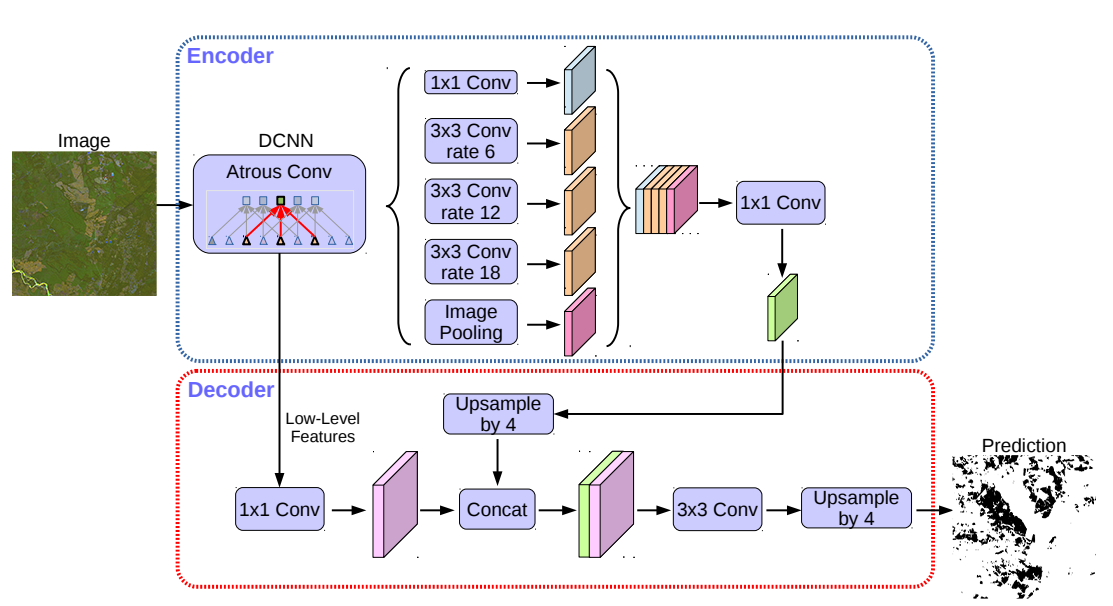
\includegraphics[width=\columnwidth]{model}
 \caption{Arquitectura DeepLabV3+ (Adaptado de \cite{chen2018})}
 \label{fig:model}
\end{figure}

Como se mencionó, la arquitectura de DeepLabV3+ se basa en un codificador que utiliza convolución \textit{atrous}, técnica heredada de DeepLabV3. Una innovación clave es la introducción de convoluciones \textit{atrous} separables, que descomponen las convoluciones en dos pasos: una convolución \textit{atrous} y una convolución punto a punto (1x1). Esto reduce significativamente los cálculos, manteniendo la eficiencia y la precisión en la segmentación.

El decodificador de DeepLabV3+ es crucial para recuperar información espacial perdida durante la codificación, mejorando la precisión de los detalles finos y los límites de los objetos. La aplicación de convoluciones separables en profundidad tanto en el módulo ASPP como en el decodificador aumenta la eficiencia computacional sin comprometer la precisión \cite{chen2018}.

Además, DeepLabV3+ mejora la segmentación en los límites de los objetos mediante técnicas avanzadas de decodificación, logrando una predicción precisa de píxeles. Su adaptabilidad a diferentes resoluciones de entrada permite ajustar el modelo según los recursos disponibles, haciéndolo aplicable desde dispositivos móviles hasta servidores.

La integración entre la red \textit{backbone} y el módulo decodificador es clave para su éxito. Mientras la \textit{backbone} actúa como codificador, el decodificador refina los resultados, especialmente en los límites de los objetos, utilizando características de bajo nivel para mejorar la precisión. Las convoluciones \textit{atrous} separables en el ASPP y el decodificador garantizan eficiencia sin sacrificar rendimiento.
